\documentclass[11pt, oneside]{article}   	% use "amsart" instead of "article" for AMSLaTeX format
\usepackage[margin=1in]{geometry}                		% See geometry.pdf to learn the layout options. There are lots.
\geometry{letterpaper}                   		% ... or a4paper or a5paper or ... 
%\geometry{landscape}                		% Activate for rotated page geometry
%\usepackage[parfill]{parskip}    		% Activate to begin paragraphs with an empty line rather than an indent
\usepackage{graphicx}				% Use pdf, png, jpg, or eps§ with pdflatex; use eps in DVI mode
								% TeX will automatically convert eps --> pdf in pdflatex		
\usepackage{amssymb}
%usepackage{undertilde}
\usepackage[numbered,framed]{matlab-prettifier}

\usepackage[T1]{fontenc}
\usepackage{mathtools}  % loads »amsmath«
\usepackage{physics}
\usepackage{listings}


\setlength{\parskip}{0.5em}

%SetFonts
\newcommand\Rey{\mbox{\textit{Re}}}

\title{\vspace{-6ex} Assignment 2- Messaging Passing Interface \\ {CSCI 596: Scientific Computing \& Visualization}  \vspace{-2ex}}
\author{Anup V Kanale}
\date{\vspace{-2ex}\today}							% Activate to display a given date or no date

\begin{document}
\maketitle \vspace{-5ex}

This assignment deals with implementing a global summation program using \texttt{MPI\_Send} \& \texttt{MPI\_receive} commands. Functionally, this is the same as using \texttt{MPI\_AllReduce}.
Since this job has to be run on the USC HPC clusters, I will first provide a minimal overview of how to run any program on the HPC cluster.
\vspace{-2ex} \section{Using the HPC cluster}
With respect to this assignment, the following files are needed to run a job on the HPC cluster--
\begin{enumerate}
	\item C code
	\item pbs file
\end{enumerate}
Firstly, compile the program using \texttt{mpicc} compiler and generate the executable. For example, \texttt{mpicc -o global global.c} complies the program \texttt{global.c} and generates the executable \texttt{global}. Once this is done, we have to queue this job to run on a given number of processors, say \texttt{np} using a \texttt{.pbs} (\textbf{P}ortable \textbf{B}atch \textbf{S}ystem). To this end, the \texttt{.pbs} file contains information regarding the path to the executable and the wall time request. 

The slightly tricky part here is that everytime I log into the hpc account, the \texttt{mpicc} compiler has to be setup using a shell script (\texttt{source /usc/usc/openmpi/default/setup.sh}), and the pbs file creates a new terminal session for the same user account. Therefore, it is important to include even the line to setup the mpi compiler. This can be done either in the pbs script, or in the \texttt{bashrc} file. The latter is recommended as mpicc will be used regularly.

Finally, submit the job using the command \texttt{qsub <filename>.pbs}. To query the status, use \texttt{qstat -u <user-name>}

\section{Global Summation using \texttt{MPI\_Send} \& \texttt{MPI\_Recv}}
This program uses the butterfly communication structure, refer to the question sheet and lecture notes on MPI for details. Each process contributes a partial value, and at the end, all the processes will have the globally summed value of these partial contributions.

%\subsection*{Use of Bitwise Logical XOR}
%
%	\begin{equation}
%	\begin{split}
%		\text{0 XOR 0 = 1}, \text{1 XOR 1 = 0} \\
%		\text{0 XOR 1 = 1}, \text{1 XOR 0 = 1}
%	\end{split}
%	\end{equation}
The source code, and the results are shown below.
	\begin{figure}
		\centering
		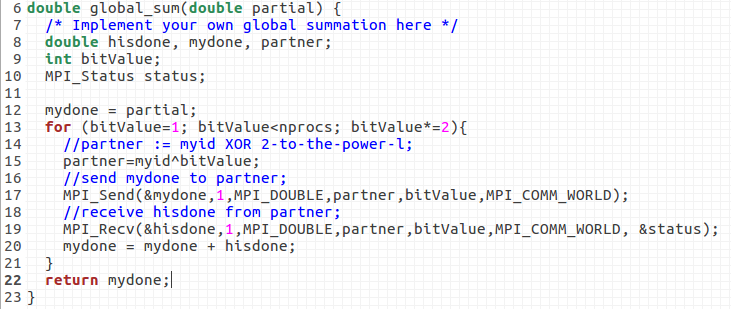
\includegraphics[scale=0.6]{globalProg.png}
		\caption{C program}
	\end{figure}
	\begin{figure}
		\centering
		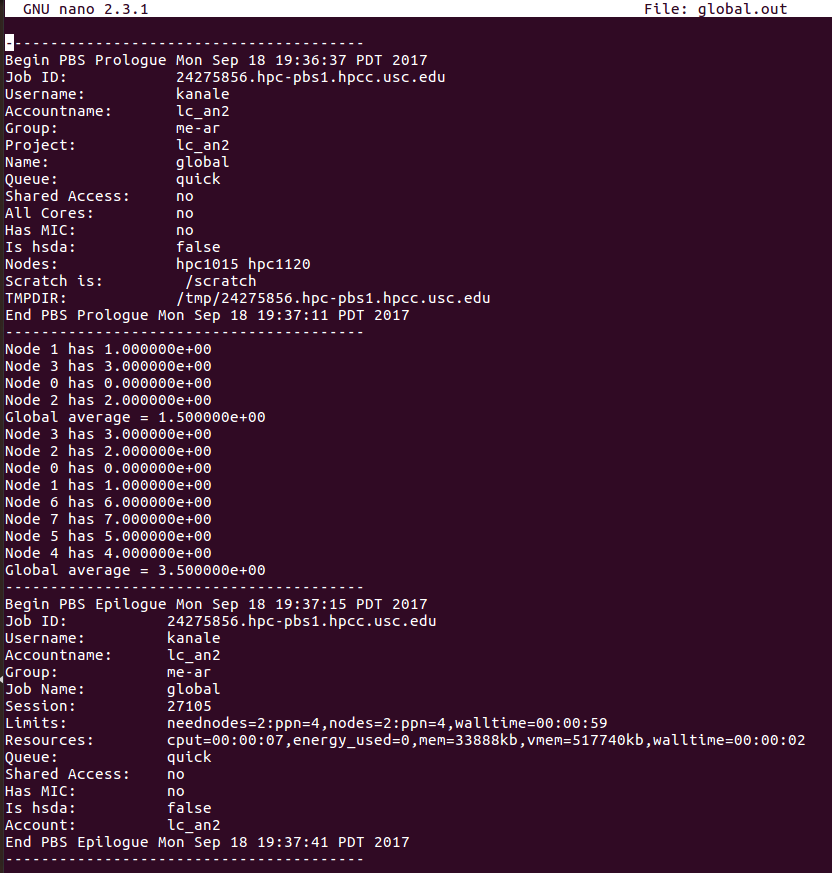
\includegraphics[scale=0.4]{globalSum.png}
		\caption{Results for running the global summation program on 4 and 8 processors}
	\end{figure}
\end{document}